\documentclass[runningheads]{llncs}

\usepackage[T5,T1]{fontenc}
\usepackage[utf8]{inputenc}
\usepackage[vietnamese]{babel}
\usepackage{amsmath}
\usepackage{amssymb}
\usepackage{graphicx}
\usepackage{booktabs}
\usepackage[protrusion=true,expansion=false]{microtype}
\usepackage{url}
\usepackage[backend=biber, style=lncs, sorting=none, giveninits=true,
    maxbibnames=6, url=false, doi=true, eprint=true, isbn=false, language=english]{biblatex}
\addbibresource{references.bib}

\setcounter{topnumber}{3}
\setcounter{bottomnumber}{2}
\setcounter{totalnumber}{4}
\renewcommand{\topfraction}{0.85}
\renewcommand{\bottomfraction}{0.85}
\renewcommand{\textfraction}{0.15}
\renewcommand{\floatpagefraction}{0.8}

\begin{document}

\title{Tăng cường chọn lọc hình ảnh dưới nước\\cho bài toán phát hiện đối tượng với YOLO11}
\titlerunning{Tăng cường chọn lọc hình ảnh dưới nước cho YOLO11}

\author{Nguyễn Quốc Bảo\inst{1} \and Phan Lê Văn Minh\inst{1}}
\authorrunning{N. Q. Bảo và P. L. V. Minh}

\institute{Trường Đại học Bách khoa, Đại học Đà Nẵng, Đà Nẵng, Việt Nam\\
    \email{\{102250412,102250417\}@hv.dut.udn.vn}}

\maketitle

\begin{abstract}
    Tăng cường ảnh dưới nước (UIE) thường được áp dụng trước bước phát hiện đối tượng. Tuy nhiên, các nghiên cứu gần đây chỉ ra rằng việc áp dụng một phương pháp tăng cường duy nhất cho mọi ảnh không giúp nâng cao độ chính xác phát hiện. Chúng tôi khảo sát giải pháp chọn lọc theo từng ảnh trên tập chuẩn RUOD với mô hình phát hiện YOLO11n. Một bộ chọn ResNet18 nhỏ gọn sẽ chọn cho mỗi ảnh giữa bản gốc, SCNet và Semi-UIR. Nhãn huấn luyện của bộ chọn được tạo bằng quy trình out-of-fold nhằm tránh việc mô hình đánh giá ảnh đã nhìn thấy khi huấn luyện. Bộ chọn đạt mAP ngang ngửa ảnh gốc do giữ nguyên bản gốc ở phần lớn các trường hợp. Chúng tôi cũng đưa vào một thử nghiệm đối chứng, trong đó oracle chọn giữa ảnh gốc và ảnh lật ngang; thử nghiệm hình học này mang lại mức tăng mAP tương đương với oracle trên các bản tăng cường quang học, cho thấy sự nhạy cảm của detector trước các biến đổi không gian đóng góp một phần vào khoảng cách oracle. Kết hợp dự đoán của 4 góc nhìn bằng phương pháp hợp nhất hộp trọng số (WBF) mang lại mức tăng nhỏ so với ảnh gốc. Cuối cùng, việc huấn luyện detector trên cả ảnh gốc lẫn ảnh tăng cường đạt mAP tương đương detector chỉ học ảnh gốc khi kiểm tra trên ảnh sạch (với cùng số lượt ảnh huấn luyện), đồng thời đạt mAP cao hơn ở 12 điều kiện suy giảm chưa từng thấy khi huấn luyện. Trong các thử nghiệm của chúng tôi, ảnh tăng cường hữu ích nhất khi đóng vai trò là dữ liệu huấn luyện đa miền nhằm nâng cao độ bền, thay vì dùng làm lựa chọn theo từng ảnh ở pha suy luận.

    \keywords{Tăng cường ảnh dưới nước \and Phát hiện đối tượng dưới nước \and Tăng cường chọn lọc \and YOLO11 \and RUOD \and UIEB.}
\end{abstract}

% ---------------------------------------------------------------------------
\section{Giới thiệu}
\label{sec:intro}

Camera gắn trên các phương tiện dưới nước tự hành (AUV) và phương tiện điều khiển từ xa (ROV) thu nhận hình ảnh chịu ảnh hưởng bởi sự hấp thụ và tán xạ ánh sáng phụ thuộc bước sóng~\cite{fuRethinkingGeneralUnderwater2023,liUnderwaterImageEnhancement2019}. Ánh sáng đỏ suy giảm nhanh chóng ở độ sâu nông. Do đó, các khung cảnh thu được thường có độ tương phản thấp, bị ám sắc xanh lam hoặc xanh lục, đường biên mờ nhạt và bị sương mù tán xạ thuận bao phủ.

Các kiến trúc học sâu dùng cho tăng cường ảnh dưới nước (UIE), chẳng hạn như SCNet~\cite{fuUnderwaterImageEnhancement2022} và Semi-UIR~\cite{huangContrastiveSemisupervisedLearning2023}, đạt chỉ số PSNR và SSIM cao khi so với ảnh tham chiếu. Thực tế phổ biến thường đặt các mô hình này ở khâu tiền xử lý phía trước detector, với giả định rằng ảnh có chất lượng thị giác sạch hơn sẽ giúp phát hiện đối tượng chính xác hơn.

Awad và cộng sự~\cite{awadRevisitingUnderwaterImage2026} đã chứng minh rằng giả định này không phải lúc nào cũng đúng. Trên nhiều họ detector khác nhau, việc áp dụng đồng loạt một phương pháp tăng cường cho tất cả các ảnh làm giảm độ chính xác phát hiện trung bình so với ảnh gốc, mặc dù một số ảnh riêng lẻ vẫn có cải thiện. Trên tập chuẩn RUOD~\cite{fuRethinkingGeneralUnderwater2023}, họ đã tính toán mức cận trên lý thuyết (mixed-set oracle) bằng cách chọn ra phiên bản tốt nhất trong số mười phiên bản (ảnh gốc và 9 bản tăng cường) cho từng ảnh nhờ vào nhãn ground-truth. Oracle này nâng mAP trung bình từng ảnh từ 0,68 lên 0,77 (+0,09).

Mức cận trên lý thuyết đó đặt ra hai câu hỏi thực tế. Thứ nhất, liệu một bộ chọn tự động có thể đưa ra quyết định chọn phiên bản thắng cuộc chỉ dựa vào các điểm ảnh gốc mà không cần nhãn ground-truth hay không? Thứ hai, bao nhiêu phần của khoảng cách oracle bắt nguồn từ việc phục hồi quang học thực sự, và bao nhiêu phần đến từ sự dao động kết quả dự đoán của detector giữa các biến thể của cùng một khung cảnh?

Chúng tôi nghiên cứu các câu hỏi này với YOLO11n~\cite{jocherUltralyticsYOLO2024} trên tập dữ liệu chuẩn RUOD gồm 14.000 ảnh. Các phiên bản ứng viên cho mỗi ảnh gồm bản gốc, SCNet và Semi-UIR. Các kết quả chính của chúng tôi gồm:
\begin{itemize}
    \item Chúng tôi xây dựng quy trình gán nhãn out-of-fold với ngưỡng biên $\delta = 0{,}01$. Bộ chọn ResNet18~\cite{heDeepResidualLearning2016} hoạt động trên ảnh đầu vào kích thước $224 \times 224$ với độ trễ 7,7\,ms mỗi khung hình.
    \item Trên 4.200 ảnh test, bộ chọn có ngưỡng biên đạt 0,6159 mAP@0.5:0.95 (thu hẹp +3,2\% khoảng cách oracle) so với 0,6155 của ảnh gốc. Bộ chọn giữ nguyên ảnh gốc ở 85,5\% các trường hợp. Sử dụng SCNet đồng loạt đạt 0,6129, Semi-UIR đạt 0,6084 và chọn ngẫu nhiên đạt 0,6120.
    \item Trong thử nghiệm đối chứng không qua tăng cường, oracle chọn giữa ảnh gốc và ảnh lật ngang đạt mức tăng mAP từng ảnh là +0,0207. Con số này tương đương 144\% mức tăng +0,0144 mà oracle giữa ảnh gốc và SCNet đạt được.
    \item Hợp nhất dự đoán trên 4 góc nhìn bằng WBF~\cite{solovyevWeightedBoxesFusion2021} mang lại mức tăng +0,0023 mAP@0.5:0.95 trên toàn bộ tập test, với khoảng tin cậy 95\% là $[+0{,}0014, +0{,}0051]$ nằm hoàn toàn trên 0.
    \item Huấn luyện đa phiên bản trên cả ảnh gốc và ảnh tăng cường nâng mAP@0.5:0.95 trên ảnh gốc từ 0,5990 lên 0,6155 so với baseline 50 epoch, ngang bằng detector huấn luyện 150 epoch trên ảnh gốc (0,6150). Mô hình này còn đạt mAP cao hơn ở cả 12 điều kiện suy giảm chưa từng thấy, dù cần xử lý gấp 3 lần lượt ảnh trong quá trình huấn luyện.
\end{itemize}

% ---------------------------------------------------------------------------
\section{Các công trình liên quan}
\label{sec:related}

\subsection{Tăng cường ảnh dưới nước}

SCNet~\cite{fuUnderwaterImageEnhancement2022} được thiết kế nhằm thích ứng với nhiều loại nước khác nhau. Tại nhiều tầng tỷ lệ của U-Net, mạng làm mất tương quan không gian qua instance whitening và chuẩn hóa thống kê kênh, giúp các đặc trưng trung gian ít phụ thuộc vào loại nước cụ thể.

Semi-UIR~\cite{huangContrastiveSemisupervisedLearning2023} giải quyết sự thiếu hụt dữ liệu huấn luyện theo cặp bằng khung mean-teacher kết hợp điều chuẩn tương phản. Một ngân hàng bộ nhớ đáng tin cậy lưu giữ các nhãn giả được lọc theo chỉ số chất lượng không cần ảnh tham chiếu. Lúc suy luận, mạng điều biến độ sáng có chú ý (AIMnet) xử lý các biểu diễn độ sáng Gaussian đa tỷ lệ.

Cả hai mô hình đều được đánh giá trên tập UIEB~\cite{liUnderwaterImageEnhancement2019} bằng PSNR và SSIM. Các chỉ số này phản ánh độ tương đồng với ảnh chụp tham chiếu chứ không đo lường hiệu quả phát hiện đối tượng ở hạ nguồn.

\subsection{Tăng cường cho bài toán phát hiện đối tượng dưới nước}

Fu và cộng sự~\cite{fuRethinkingGeneralUnderwater2023} giới thiệu tập RUOD cho bài toán phát hiện dưới nước, ghi nhận tác động không đồng nhất giữa các phương pháp tăng cường thông thường và các họ detector. Luo và cộng sự~\cite{luoMASYOLOv11ImprovedUnderwater2025} đề xuất MAS-YOLOv11 với các đầu chú ý đa tỷ lệ cho các khung cảnh dưới nước phức tạp. Huang và cộng sự~\cite{huangAMIEODAdaptiveMultiExperts2026} phát triển AMIEOD để định tuyến linh hoạt các ảnh thiếu sáng qua các module chuyên gia tăng cường.

Awad và cộng sự~\cite{awadRevisitingUnderwaterImage2026} so sánh 9 bộ tăng cường trên các detector hiện đại. Việc áp dụng đồng loạt bất kỳ bộ tăng cường nào đều không vượt qua được ảnh gốc trên toàn bộ tập test. Họ đưa ra phân tích cận trên oracle từng ảnh, nhưng phương pháp này đòi hỏi nhãn test và các detector được huấn luyện riêng biệt cho từng miền.

\subsection{Hợp nhất hộp và tăng cường lúc kiểm thử}

Tăng cường lúc kiểm thử (TTA) kết hợp các dự đoán thu được từ nhiều góc nhìn biến đổi của ảnh đầu vào. Non-maximum suppression (NMS) thông thường giữ lại một hộp có độ tin cậy cao nhất trong cụm và loại bỏ các hộp chồng lấn. Phương pháp hợp nhất hộp trọng số (WBF)~\cite{solovyevWeightedBoxesFusion2021} thay vào đó gom cụm các hộp chồng lấn và tính tọa độ trung bình có trọng số theo độ tin cậy.

% ---------------------------------------------------------------------------
\section{Phương pháp}
\label{sec:method}

\subsection{Tổng quan hệ thống}

Gọi $x \in \mathbb{R}^{H \times W \times 3}$ là một khung hình RGB dưới nước. Chúng tôi sử dụng hai mô hình tăng cường công khai với trọng số do tác giả cung cấp: SCNet ($E_{\mathrm{SC}}$) và Semi-UIR ($E_{\mathrm{SU}}$). Tập các phiên bản ứng viên gồm:
\begin{equation}
    \mathcal{V}(x) = \{\, v_0, v_1, v_2 \,\} = \{\, x,\; E_{\mathrm{SC}}(x),\; E_{\mathrm{SU}}(x) \,\}.
\end{equation}
Bộ chọn $f_\theta$ nhận ảnh gốc $x$ và đưa ra chỉ số $\hat{k} \in \{0, 1, 2\}$. Phiên bản được chọn $v_{\hat{k}}$ sau đó được đưa vào detector YOLO11n ($D$) đã tinh chỉnh. Hình~\ref{fig:sample_enhancement} minh họa ảnh mẫu dưới nước trước và sau khi tăng cường với Semi-UIR và SCNet. Quy trình tổng thể, bao gồm việc sinh nhãn out-of-fold và suy luận chọn lọc, được thể hiện ở Hình~\ref{fig:pipeline}.

\begin{figure}[t]
    \centering
    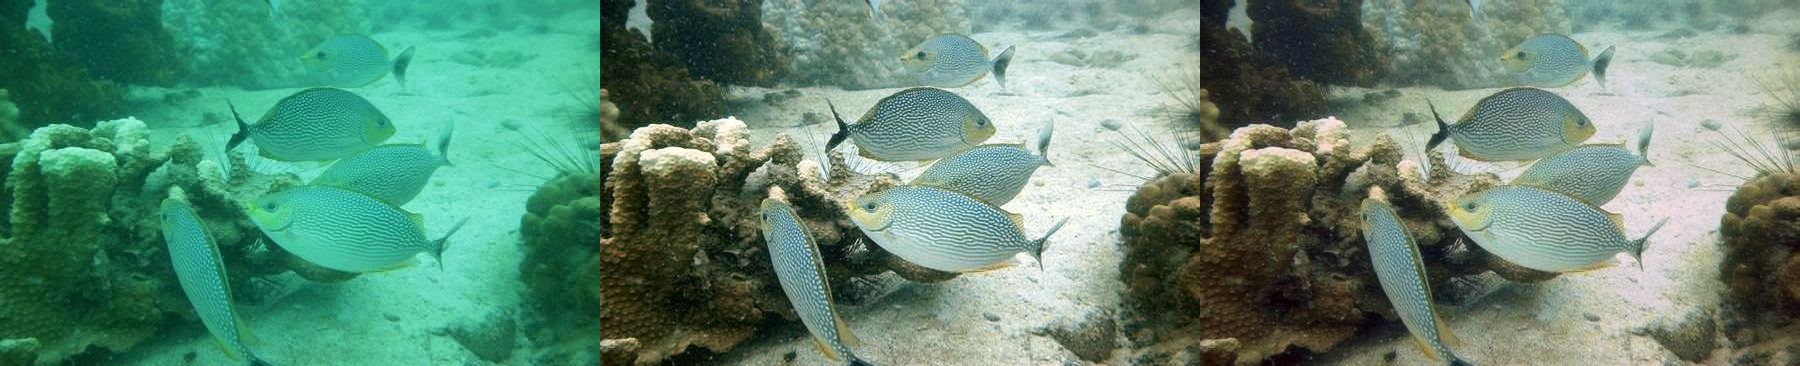
\includegraphics[width=\textwidth]{figures/sample_enhancement.png}
    \caption{Ảnh mẫu trước và sau khi tăng cường. Từ trái sang phải: ảnh gốc đầu vào, Semi-UIR và SCNet.}
    \label{fig:sample_enhancement}
\end{figure}

\begin{figure}[t]
    \centering
    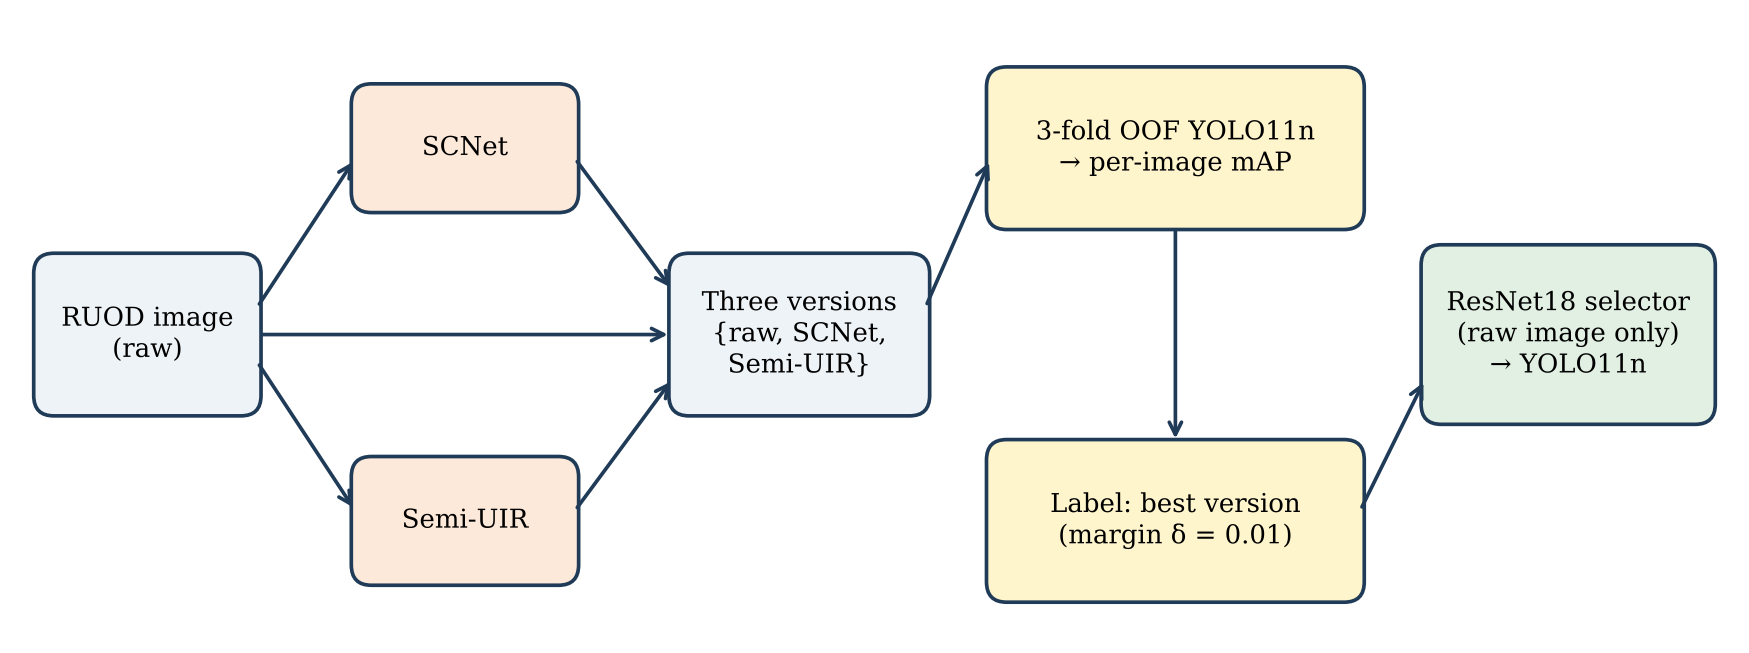
\includegraphics[width=\textwidth]{figures/pipeline_en.png}
    \caption{Quy trình tổng thể (Pipeline). Mỗi ảnh huấn luyện được tăng cường bởi SCNet và Semi-UIR; các detector YOLO11n out-of-fold chấm điểm cả ba phiên bản trên từng ảnh; phiên bản tốt nhất (với biên độ $\delta$) trở thành nhãn mục tiêu cho bộ chọn ResNet18 vốn chỉ nhìn thấy ảnh gốc.}
    \label{fig:pipeline}
\end{figure}

\subsection{Bộ tăng cường và quy trình xử lý}
\label{sec:method-enh}

Cả hai bộ tăng cường đều chạy ở độ phân giải gốc (cạnh dài 640\,px) với trọng số phát hành.
\begin{itemize}
    \item \textbf{SCNet:} Giữ lại nhánh giải mã tăng cường và loại bỏ mạng phụ VGG16 (vốn dùng làm hàm mất mát tri giác khi train). Ảnh đầu vào được đệm phản xạ thành bội số của 8, đầu ra được cắt về kích thước ban đầu và lượng tử hóa về $[0, 255]$.
    \item \textbf{Semi-UIR:} Bản đồ độ sáng $L(x)$ được tính bằng cách tích chập kênh độ sáng với các kernel Gaussian ở $\sigma \in \{15, 60, 90\}$, lấy trung bình logarit và chuẩn hóa về $[0, 255]$. Đầu vào và bản đồ độ sáng được đệm phản xạ thành bội số của 16. Thời gian xử lý trung bình khoảng 2\,s mỗi ảnh.
\end{itemize}
Các ảnh tăng cường được lưu dưới dạng JPEG ($\text{quality} = 95$) và dùng chung nhãn hộp với ảnh gốc.

\subsection{Quy trình gán nhãn Out-of-Fold (OOF) cho bộ chọn}
\label{sec:method-labels}

Detector đã học trên một ảnh thường cho điểm quá cao trên chính ảnh đó, làm sai lệch nhãn mục tiêu của bộ chọn. Do đó, chúng tôi áp dụng quy trình out-of-fold 3-fold:
\begin{enumerate}
    \item 9.800 ảnh train RUOD được chia thành 3 fold $\mathcal{F}_0, \mathcal{F}_1, \mathcal{F}_2$ với seed 0 (mã hash MD5: \texttt{ea44b385539c}).
    \item Với mỗi fold $k \in \{0, 1, 2\}$, huấn luyện một detector YOLO11n trong 30 epoch trên cả 3 phiên bản của 2 fold còn lại ($\approx 19.600$ ảnh).
    \item Dùng checkpoint \texttt{last.pt} để dự đoán trên cả 3 phiên bản của fold bị giữ lại $\mathcal{F}_k$ ($\text{conf} = 0{,}001$, $\text{IoU} = 0{,}7$).
    \item Dùng \texttt{pycocotools} để tính mAP@0.5:0.95 từng ảnh $m_{i,0}, m_{i,1}, m_{i,2}$. Ảnh không có nhãn nhận điểm 0.
\end{enumerate}
Với biên độ chênh lệch $\delta = 0{,}01$, nhãn mục tiêu $y_i$ được gán như sau:
\begin{equation}
    y_i =
    \begin{cases}
        0                    & \text{nếu } \max_{k \in \{1, 2\}} m_{i,k} - m_{i,0} < \delta, \\
        \arg\max_{k} m_{i,k} & \text{ngược lại}.
    \end{cases}
\end{equation}

\subsection{Kiến trúc bộ chọn và quy tắc quyết định}

Bộ chọn sử dụng ResNet18~\cite{heDeepResidualLearning2016} tiền huấn luyện trên ImageNet với đầu tuyến tính 3 ngõ ra. Đầu vào là ảnh gốc kích thước $224 \times 224 \times 3$ (chi phí 7,7\,ms trên GPU NVIDIA Tesla T4). Chúng tôi huấn luyện theo hai hàm mục tiêu:
\begin{itemize}
    \item \textbf{Cross-entropy có trọng số lớp (\texttt{ce}):}
          \begin{equation}
              \mathcal{L}_{\mathrm{ce}} = -\sum_{c=0}^2 w_c \cdot \mathbb{I}(y = c) \log p_c,
          \end{equation}
          trong đó $w_c$ là nghịch đảo tần suất xuất hiện của lớp.
    \item \textbf{Hồi quy mAP (\texttt{reg}):} mạng dự đoán 3 giá trị mAP $(\hat{m}_0, \hat{m}_1, \hat{m}_2)$ dưới hàm mất mát Smooth L1.
\end{itemize}

\subsubsection{Ngưỡng quyết định ($\tau$)}
Để tránh gọi tăng cường không cần thiết, chọn $k^* = \arg\max_{k \in \{1, 2\}} p_k$ chỉ khi $p_{k^*} - p_0 > \tau$; ngược lại, giữ nguyên ảnh gốc. Với mô hình hồi quy, điều kiện là $\hat{m}_{k^*} - \hat{m}_0 > \tau$.

\subsubsection{Tiêu chí chọn mô hình trên tập kiểm thực (validation)}
Luôn chọn ảnh gốc đã đạt độ chính xác 58,2\% trên nhãn train và 62,4\% trên nhãn test. Vì vậy, độ chính xác phân loại thông thường là thước đo không phù hợp. Việc chọn mô hình và tinh chỉnh ngưỡng dựa trên chosen-mAP trên tập val 20\% giữ lại (1.960 ảnh):
\begin{equation}
    \text{chosen-mAP} = \frac{1}{N_{\mathrm{val}}} \sum_{i=1}^{N_{\mathrm{val}}} m_{i, \hat{y}_i}.
\end{equation}
Các ngưỡng tối ưu tìm được là $\tau = 0{,}625$ cho \texttt{ce} và $\tau = 0{,}040$ cho \texttt{reg}.

\subsection{Đánh giá bằng cách ghép dự đoán đã lưu}

Đánh giá trên 4.200 ảnh test RUOD gồm 4 bước:
\begin{enumerate}
    \item Huấn luyện một detector duy nhất (\texttt{full.pt}) trong 50 epoch trên cả 3 phiên bản của 9.800 ảnh train (tổng cộng 29.400 ảnh, thời gian 10.732\,s).
    \item Dự đoán trước trên toàn bộ các phiên bản và lưu trữ kết quả. Mỗi chính sách được chấm điểm bằng cách ghép các dự đoán tương ứng và chạy \texttt{pycocotools}.
    \item Lấy mẫu lại paired bootstrap 1.000 lần để tính khoảng tin cậy 95\% và p-value $p_{\text{boot}}(\Delta \le 0)$ cho hiệu mAP từng ảnh so với mốc ảnh gốc.
    \item Tỷ lệ khoảng cách oracle được thu hẹp tính bằng:
          \begin{equation}
              G = \frac{\mathrm{mAP}_{\text{chính\_sách}} - \mathrm{mAP}_{\text{gốc}}}{\mathrm{mAP}_{\mathrm{oracle}} - \mathrm{mAP}_{\text{gốc}}} \times 100\%.
          \end{equation}
\end{enumerate}

\subsection{Thử nghiệm đối chứng Oracle với ảnh lật ngang}
\label{sec:method-noise}

Để kiểm tra xem mức tăng của oracle bắt nguồn từ chất lượng quang học hay từ sự dao động của detector, chúng tôi thêm nhóm đối chứng dựa trên phép lật ngang $T_{\mathrm{flip}}$. Với đầu vào $x$, các dự đoán trên $T_{\mathrm{flip}}(x)$ được ánh xạ ngược về tọa độ gốc qua $T_{\mathrm{flip}}^{-1}$. Ảnh lật có cùng màu sắc và độ tương phản với ảnh gốc. Sự chênh lệch giữa $m_{i, \mathrm{orig}}$ và $m_{i, \mathrm{flip}}$ thuần túy phản ánh độ nhạy không gian của detector và thuật toán NMS. Định nghĩa:
\begin{equation}
    \text{Oracle}_{\{\mathrm{orig}, \mathrm{flip}\}}(i) = \max \left( m_{i, \mathrm{orig}},\; m_{i, \mathrm{flip}} \right).
\end{equation}
Nếu nhóm đối chứng này đạt mức tăng tương đương oracle quang học, điều đó chứng minh một phần mức tăng oracle đến từ sự dao động của detector chứ không phải từ phép tăng cường.

\subsection{Hợp nhất hộp đa góc nhìn bằng WBF}
\label{sec:method-wbf}

Chúng tôi hợp nhất các hộp dự đoán trên 4 góc nhìn (gốc, lật, SCNet, Semi-UIR) bằng WBF~\cite{solovyevWeightedBoxesFusion2021} với các tham số cố định: $\text{IoU}_{\mathrm{thr}} = 0{,}6$, $\text{skip\_box\_thr} = 0{,}001$, tối đa 150 hộp mỗi góc nhìn.

% ---------------------------------------------------------------------------
\section{Thiết lập thực nghiệm}
\label{sec:setup}

\subsection{Tập dữ liệu}

\textbf{UIEB}~\cite{liUnderwaterImageEnhancement2019} gồm 890 ảnh dưới nước chụp thực tế theo cặp. Chúng tôi sử dụng tập test chuẩn gồm 90 ảnh ở độ phân giải gốc để kiểm chứng các chỉ số phục hồi công bố.

\textbf{RUOD}~\cite{fuRethinkingGeneralUnderwater2023} chứa 14.000 ảnh dưới nước (9.800 train, 4.200 test) thuộc 10 lớp đối tượng: \emph{hải sâm (holothurian), nhím biển (echinus), sò điệp (scallop), sao biển (starfish), cá (fish), san hô (corals), thợ lặn (diver), mực (cuttlefish), rùa biển (turtle), sứa (jellyfish)}. Cạnh dài của ảnh được đưa về 640\,px.

\subsection{Chi tiết cài đặt}

Thực nghiệm chạy trên Kaggle với 2 GPU NVIDIA Tesla T4, PyTorch 2.11 (CUDA 12.8) và Ultralytics 8.4.174. YOLO11n sử dụng kích thước $640 \times 640$, batch size 32, seed 0. ResNet18 được huấn luyện 15 epoch bằng AdamW (learning rate $3 \times 10^{-4}$, weight decay $10^{-4}$) trên tập train/val tỷ lệ 80/20 (7.840 train, 1.960 val).

\subsection{Thước đo}

PSNR và SSIM tính qua \texttt{scikit-image}. Độ chính xác phát hiện là COCO mAP@0.5 và mAP@0.5:0.95 từ \texttt{pycocotools}. Khoảng tin cậy là khoảng 95\% paired bootstrap qua 1.000 lần lấy mẫu lại.

% ---------------------------------------------------------------------------
\section{Kết quả và thảo luận}
\label{sec:results}

\subsection{Kiểm chứng bộ tăng cường trên UIEB}
\label{sec:res-uieb}

Bảng~\ref{tab:uieb} so sánh kết quả đo đạc trên 90 ảnh test UIEB với số liệu công bố. PSNR của SCNet lệch trong khoảng 0,35\,dB và Semi-UIR lệch 0,38\,dB so với công bố. SSIM chênh lệch dưới 0,02. Cả hai bộ tăng cường đều nâng PSNR hơn 4,5\,dB so với ảnh gốc.

\begin{table}[t]
    \centering
    \caption{PSNR và SSIM trên tập test UIEB (90 ảnh, trung bình $\pm$ độ lệch chuẩn).}
    \label{tab:uieb}
    \setlength{\tabcolsep}{4pt}
    \begin{tabular}{l c c c c}
        \toprule
                                                                   & \multicolumn{2}{c}{Kết quả đo đạc}  & \multicolumn{2}{c}{Công bố}                  \\
        Phương pháp                                                & PSNR (dB)                           & SSIM                          & PSNR  & SSIM   \\
        \midrule
        Ảnh gốc                                                    & $17{,}90 \pm 5{,}35$                & $0{,}776 \pm 0{,}137$         & --    & --     \\
        SCNet~\cite{fuUnderwaterImageEnhancement2022}              & $22{,}43 \pm 4{,}43$                & $0{,}879 \pm 0{,}082$         & 22,08 & 0,8625 \\
        Semi-UIR~\cite{huangContrastiveSemisupervisedLearning2023} & $\mathbf{24{,}21} \pm 4{,}03$       & $\mathbf{0{,}886} \pm 0{,}069$& 24,59 & 0,9010 \\
        \midrule
        Oracle từng ảnh$^{\dagger}$                                & 24,95                               & 0,9006                        & --    & --     \\
        \bottomrule
        \multicolumn{5}{l}{\footnotesize $^{\dagger}$Phiên bản tốt nhất được chọn độc lập cho từng chỉ số trên mỗi ảnh.}
    \end{tabular}
\end{table}

\begin{table}[t]
    \centering
    \caption{Số ảnh test UIEB (trên 90 ảnh) đạt điểm cao nhất theo từng chỉ số.}
    \label{tab:best}
    \begin{tabular}{l c c c}
        \toprule
        Chỉ số & Ảnh gốc & SCNet & Semi-UIR \\
        \midrule
        PSNR   & 6       & 24    & 60       \\
        SSIM   & 10      & 29    & 51       \\
        \bottomrule
    \end{tabular}
\end{table}

Không có phương pháp nào thắng trên mọi bức ảnh (Bảng~\ref{tab:best}). Theo PSNR, Semi-UIR tốt nhất ở 60 ảnh, SCNet ở 24 ảnh, ảnh gốc ở 6 ảnh. Oracle đạt 24,95\,dB PSNR và 0,9006 SSIM. Trên ảnh 703, ảnh gốc đạt 40,63\,dB, trong khi SCNet và Semi-UIR tụt xuống 27,54\,dB và 26,38\,dB. Ngược lại, trên ảnh 713, ảnh gốc chỉ đạt 9,75\,dB, trong khi SCNet đạt 19,64\,dB và Semi-UIR đạt 28,54\,dB.

\subsection{Nhãn Out-of-Fold trên tập train RUOD}
\label{sec:res-oof}

Quy trình out-of-fold trên 9.800 ảnh train tạo ra 5.704 nhãn gốc (58,2\%), 2.208 nhãn SCNet (22,5\%) và 1.888 nhãn Semi-UIR (19,3\%).

Trên các dự đoán out-of-fold này, ảnh gốc đạt 0,5808 mAP@0.5:0.95 (0,6873 tính từng ảnh). Áp dụng SCNet đồng loạt đạt 0,5785 (0,6859 từng ảnh) và Semi-UIR đồng loạt đạt 0,5729 (0,6817 từng ảnh). Oracle out-of-fold đạt 0,7164 mAP từng ảnh (+0,0291 so với ảnh gốc).

\subsection{Kết quả phát hiện trên tập test RUOD}
\label{sec:res-detection}

Bảng~\ref{tab:ruod} tổng hợp kết quả của các chính sách trên 4.200 ảnh test RUOD dưới cùng một detector.

\begin{table}[t]
    \centering
    \caption{Hiệu năng phát hiện đối tượng trên tập test RUOD (4.200 ảnh) với YOLO11n.}
    \label{tab:ruod}
    \resizebox{\columnwidth}{!}{
        \begin{tabular}{l c c c c c c c}
            \toprule
            Chính sách                           & mAP@0.5         & mAP@0.5:0.95    & mAP từng ảnh    & Gap thu hẹp (Toàn tập / Từng ảnh) & $\Delta$ so với Gốc [CI 95\%]       & $p_{\text{boot}}(\Delta \le 0)$ & Tỷ lệ chọn (Gốc / SC / Semi) \\
            \midrule
            Luôn chọn gốc (\texttt{orig})        & 0,8468          & 0,6155          & 0,7186          & 0,0\% / 0,0\%            & -- (Mốc)                            & --                              & 4200 / 0 / 0                 \\
            Luôn chọn SCNet                      & 0,8449          & 0,6129          & 0,7154          & -18,1\% / -13,6\%        & -0,0031 [-0,0049; -0,0013]          & 1,000                           & 0 / 4200 / 0                 \\
            Luôn chọn Semi-UIR                   & 0,8422          & 0,6084          & 0,7130          & -50,0\% / -24,2\%        & -0,0056 [-0,0077; -0,0034]          & 1,000                           & 0 / 0 / 4200                 \\
            Chọn ngẫu nhiên                      & 0,8444          & 0,6120          & 0,7148          & -24,7\% / -16,3\%        & -0,0038 [-0,0054; -0,0021]          & 1,000                           & 1387 / 1401 / 1412           \\
            \midrule
            Bộ chọn \texttt{ce}                  & 0,8472          & 0,6146          & 0,7173          & -6,4\% / -5,4\%          & -0,0012 [-0,0025; 0,0000]           & 0,970                           & 2210 / 1101 / 889            \\
            \textbf{Bộ chọn \texttt{ce+$\tau$}}  & \textbf{0,8474} & \textbf{0,6159} & 0,7182          & \textbf{+3,2\%} / -1,5\% & \textbf{-0,0004 [-0,0010; +0,0003]} & 0,851                           & \textbf{3593 / 319 / 288}    \\
            Bộ chọn \texttt{reg}                 & 0,8457          & 0,6142          & 0,7182          & -8,8\% / -1,7\%          & -0,0004 [-0,0018; +0,0009]          & 0,734                           & 2133 / 1373 / 694            \\
            Bộ chọn \texttt{reg+$\tau$}          & 0,8462          & 0,6146          & 0,7183          & -5,9\% / -1,4\%          & -0,0003 [-0,0014; +0,0008]          & 0,745                           & 3019 / 828 / 353             \\
            \midrule
            Oracle$^{\dagger}$                   & \textbf{0,8524} & \textbf{0,6296} & \textbf{0,7417} & 100,0\% / 100,0\%        & +0,0231 [+0,0216; +0,0247]          & 0,000                           & 2620 / 846 / 734             \\
            \bottomrule
            \multicolumn{8}{l}{\footnotesize $^{\dagger}$Oracle được đánh giá với ngưỡng biên gán nhãn $\delta = 0{,}01$ (mặc định chọn gốc nếu bản tăng cường không hơn ít nhất $\delta$).}
        \end{tabular}
    }
\end{table}

\begin{table}[t]
    \centering
    \caption{Hiệu năng trên 1.960 ảnh kiểm thực giữ lại và ma trận nhầm lẫn test của Bộ chọn \texttt{ce+$\tau$} trên 4.200 ảnh test.}
    \label{tab:confusion}
    \resizebox{\columnwidth}{!}{
        \begin{tabular}{l c c c c}
            \toprule
            \multicolumn{5}{c}{\textbf{A. Hiệu năng tập kiểm thực (1.960 ảnh)}}                                                              \\
            Biến thể                       & $\tau$                    & Chosen-mAP          & \multicolumn{2}{c}{Gap thu hẹp}               \\
            \midrule
            Luôn chọn gốc                  & --                        & 0,6924              & \multicolumn{2}{c}{0,0\%}                     \\
            \texttt{ce}                    & 0                         & 0,6923              & \multicolumn{2}{c}{-0,4\%}                    \\
            \textbf{\texttt{ce+$\tau$}}    & \textbf{0,625}            & \textbf{0,6931}     & \multicolumn{2}{c}{\textbf{+2,5\%}}           \\
            \texttt{reg}                   & 0                         & 0,6918              & \multicolumn{2}{c}{-2,4\%}                    \\
            \texttt{reg+$\tau$}            & 0,040                     & 0,6931              & \multicolumn{2}{c}{+2,2\%}                    \\
            Oracle                         & --                        & 0,7202              & \multicolumn{2}{c}{100,0\%}                   \\
            \midrule
            \multicolumn{5}{c}{\textbf{B. Ma trận nhầm lẫn tập test (Hàng: Nhãn Oracle, Cột: Dự đoán)}}                                      \\
            Nhãn Oracle ($\delta = 0{,}01$)& Dự đoán Gốc               & Dự đoán SCNet       & Dự đoán Semi-UIR                    & Tổng     \\
            \midrule
            Gốc (\texttt{orig})            & \textbf{2.259} (86,2\%)   & 176 (6,7\%)         & 185 (7,1\%)                         & 2.620    \\
            SCNet                          & 708 (83,7\%)              & \textbf{83} (9,8\%) & 55 (6,5\%)                          & 846      \\
            Semi-UIR                       & 626 (85,3\%)              & 60 (8,2\%)          & \textbf{48} (6,5\%)                 & 734      \\
            \midrule
            Tổng dự đoán                   & 3.593 (85,5\%)            & 319 (7,6\%)         & 288 (6,9\%)                         & 4.200    \\
            \bottomrule
        \end{tabular}
    }
\end{table}

\begin{table}[t]
    \centering
    \caption{AP@0.5:0.95 theo từng lớp của các chính sách đầu vào trên tập test RUOD.}
    \label{tab:perclass}
    \resizebox{\columnwidth}{!}{
        \begin{tabular}{l c c c c c}
            \toprule
            Lớp                   & Gốc             & SCNet           & Semi-UIR        & Bộ chọn \texttt{ce+$\tau$}  & Oracle          \\
            \midrule
            hải sâm (holothurian) & 0,4966          & 0,4910          & 0,4877          & 0,4966                      & 0,5102          \\
            nhím biển (echinus)   & 0,5305          & 0,5250          & 0,5187          & 0,5298                      & 0,5446          \\
            sò điệp (scallop)     & 0,4957          & 0,4941          & 0,4791          & 0,4958                      & 0,5058          \\
            sao biển (starfish)   & 0,5508          & 0,5409          & 0,5431          & 0,5506                      & 0,5652          \\
            cá (fish)             & 0,5198          & 0,5196          & 0,5181          & 0,5191                      & 0,5337          \\
            san hô (corals)       & 0,5386          & 0,5367          & 0,5338          & 0,5377                      & 0,5519          \\
            thợ lặn (diver)       & 0,7456          & 0,7467          & 0,7397          & 0,7462                      & 0,7638          \\
            mực (cuttlefish)      & 0,8360          & 0,8320          & 0,8315          & 0,8361                      & 0,8487          \\
            rùa biển (turtle)     & 0,8383          & 0,8390          & 0,8330          & 0,8384                      & 0,8518          \\
            sứa (jellyfish)       & 0,6026          & 0,6041          & 0,5991          & \textbf{0,6089}             & 0,6208          \\
            \midrule
            Trung bình            & \textbf{0,6155} & \textbf{0,6129} & \textbf{0,6084} & \textbf{0,6159}             & \textbf{0,6296} \\
            \bottomrule
        \end{tabular}
    }
\end{table}

\subsubsection{Tăng cường đồng loạt}
Áp dụng SCNet đồng loạt làm giảm mAP@0.5:0.95 đi 0,0026 ($-0{,}0031$ từng ảnh, CI $[-0{,}0049, -0{,}0013]$). Semi-UIR làm giảm 0,0071 ($-0{,}0056$ từng ảnh, CI $[-0{,}0077, -0{,}0034]$). Cả hai khoảng tin cậy đều nằm dưới 0 ($p_{\text{boot}} = 1{,}000$). Chọn ngẫu nhiên làm giảm 0,0038 mAP từng ảnh.

\subsubsection{Độ chính xác của bộ chọn}
Bộ chọn không có ngưỡng (\texttt{ce} và \texttt{reg}) bị giảm độ chính xác do gọi tăng cường ở các ảnh không có lợi. Thêm ngưỡng $\tau = 0{,}625$ giúp Bộ chọn \texttt{ce+$\tau$} đạt 0,6159 mAP@0.5:0.95 (+3,2\% gap được thu hẹp), sát mốc 0,6155 của ảnh gốc. Khoảng tin cậy 95\% của hiệu từng ảnh là $[-0{,}0010, +0{,}0003]$ chứa 0 ($p_{\text{boot}} = 0{,}851$).

\subsubsection{Ma trận nhầm lẫn}
Bảng~\ref{tab:confusion} trình bày điểm val và ma trận nhầm lẫn trên tập test. Độ chính xác phân loại test là 56,9\%, thấp hơn mức 62,4\% nếu luôn chọn ảnh gốc. Dưới ngưỡng biên $\delta = 0{,}01$, SCNet là phương pháp thắng trên 846 ảnh test (20,1\%); bộ chọn đoán đúng SCNet ở 83 ảnh (độ nhạy 9,8\%). Semi-UIR thắng trên 734 ảnh (17,5\%); bộ chọn đoán đúng ở 48 ảnh (độ nhạy 6,5\%). Khi không áp ngưỡng $\delta$, so sánh cặp cho thấy SCNet vượt ảnh gốc ở 31,6\% số ảnh (1.327 ảnh), và Semi-UIR vượt ở 31,7\% (1.331 ảnh).

Bộ chọn duy trì điểm tương đương ảnh gốc chủ yếu nhờ ngưỡng $\tau = 0{,}625$ giữ lại ảnh gốc ở 85,5\% trường hợp (3.593 ảnh). Thời gian xử lý là 7,7\,ms mỗi ảnh.

\subsubsection{Kết quả theo lớp}
Bảng~\ref{tab:perclass} liệt kê AP cho từng lớp trong 10 lớp. Ở các lớp \emph{hải sâm}, \emph{nhím biển} và \emph{sò điệp}, bộ chọn bám sát mốc ảnh gốc. Chênh lệch lớn nhất nằm ở lớp \emph{sứa} (0,6089 so với 0,6026), đây là biến động riêng lẻ của một lớp chưa được đánh giá khoảng tin cậy riêng.

\subsection{Mức tăng Oracle khi có và không có tăng cường}
\label{sec:res-noise}

Bảng~\ref{tab:noise} so sánh các cấu hình oracle trên 4.200 ảnh test.

\begin{table}[t]
    \centering
    \caption{So sánh Oracle giữa bộ tăng cường quang học và ảnh lật ngang trên tập test RUOD.}
    \label{tab:noise}
    \resizebox{\columnwidth}{!}{
        \begin{tabular}{l c c c c}
            \toprule
            Tập ứng viên Oracle                                    & Kích thước & mAP@0.5:0.95 & $\Delta$ từng ảnh [CI 95\%] & \% Không chọn gốc \\
            \midrule
            $\{\text{gốc}, \text{gốc chạy lại}\}$                  & 2          & 0,6159       & +0,0005 [+0,0003; +0,0006]  & 2,3\%             \\
            $\{\text{gốc}, \text{scnet}\}$                         & 2          & 0,6250       & +0,0144 [+0,0133; +0,0154]  & 31,6\%            \\
            $\{\text{gốc}, \text{semiuir}\}$                       & 2          & 0,6250       & +0,0164 [+0,0150; +0,0179]  & 31,7\%            \\
            $\{\text{gốc}, \text{lật}\}$ (đối chứng)               & 2          & 0,6300       & +0,0207 [+0,0193; +0,0221]  & 38,5\%            \\
            \midrule
            Oracle UIE (gốc, SCNet, Semi-UIR)$^{\dagger}$          & 3          & 0,6300       & +0,0234 [+0,0219; +0,0250]  & 44,2\%            \\
            $\{\text{gốc}, \text{lật}, \text{SC}, \text{Semi}\}$   & 4          & 0,6386       & +0,0353 [+0,0336; +0,0371]  & 58,6\%            \\
            \bottomrule
            \multicolumn{5}{l}{\footnotesize $^{\dagger}$Oracle thuần không có ngưỡng ($\delta = 0$). Ở Bảng~\ref{tab:ruod}, oracle áp dụng ngưỡng $\delta = 0{,}01$, đạt 0,6296 mAP và 37,6\% lượt chọn phi-gốc.}
        \end{tabular}
    }
\end{table}

Oracle giữa ảnh gốc và ảnh lật ngang đạt 0,6300 mAP@0.5:0.95, ngang bằng oracle quang học thuần 3 phiên bản ($\{\text{gốc}, \text{SC}, \text{Semi}\}$). Tính theo từng ảnh, oracle ảnh lật tăng +0,0207, tương đương 144\% mức tăng của SCNet (+0,0144). Oracle 3 phiên bản đạt +0,0234 từng ảnh. Do ảnh lật không hề qua bộ tăng cường nào, phần tăng này hoàn toàn bắt nguồn từ phản ứng của detector trước tọa độ bị lật đối xứng.

Khi có 4 ứng viên (gốc, lật, SCNet, Semi-UIR), oracle đạt 0,6386. Kỳ vọng cực đại của nhiều biến ngẫu nhiên luôn tăng theo số lượng ứng viên. Do đó, việc bổ sung thêm ứng viên sẽ mở rộng biên độ oracle bất kể ứng viên đó có mang lại thông tin thị giác mới hay không.

Ở Bảng~\ref{tab:ruod}, oracle áp dụng ngưỡng $\delta = 0{,}01$, chọn bản tăng cường ở 37,6\% số ảnh (1.580 ảnh) và đạt 0,6296 mAP. Trong Bảng~\ref{tab:noise}, oracle thuần ($\delta = 0$) lấy giá trị lớn nhất tuyệt đối, chọn bản phi-gốc ở 44,2\% số ảnh và đạt 0,6300 mAP.

Nhãn mục tiêu của bộ chọn lấy từ đánh giá out-of-fold. Độ tương quan giữa mức tăng của ảnh lật và mức tăng của SCNet là 0,306. Khi nhãn mục tiêu chứa đựng nhiều sự dao động ngẫu nhiên của detector, một bộ phân loại chỉ nhìn điểm ảnh gốc sẽ gặp khó khăn khi học, điều này lý giải kết quả của bộ chọn ở trên.

\subsection{Hợp nhất hộp và lựa chọn dựa trên độ tin cậy}
\label{sec:res-fusion}

Bảng~\ref{tab:fusion} đánh giá các phương pháp hoạt động không cần nhãn ground-truth lúc test.

\begin{table}[t]
    \centering
    \caption{Hợp nhất đa góc nhìn và chọn theo độ tin cậy trên tập test RUOD.}
    \label{tab:fusion}
    \resizebox{\columnwidth}{!}{
        \begin{tabular}{l c c c}
            \toprule
            Phương pháp                        & mAP@0.5:0.95    & $\Delta$ Toàn tập & $\Delta$ Từng ảnh [CI 95\%]         \\
            \midrule
            Mốc ảnh gốc                        & 0,6155          & --                & --                                  \\
            WBF(gốc, lật)                      & 0,6145          & -0,0009           & -0,0002 [-0,0019; +0,0014]          \\
            WBF(gốc, SCNet)                    & 0,6085          & -0,0070           & -0,0050 [-0,0065; -0,0035]          \\
            WBF(gốc, SCNet, Semi-UIR)          & 0,6111          & -0,0044           & -0,0025 [-0,0044; -0,0007]          \\
            \textbf{WBF(gốc, lật, SC, Semi)}   & \textbf{0,6177} & \textbf{+0,0023}  & \textbf{+0,0032 [+0,0014; +0,0051]} \\
            \midrule
            Độ tin cậy \texttt{conf\_top5}     & 0,6129          & -0,0025           & -0,0021 [-0,0035; -0,0006]          \\
            Độ tin cậy \texttt{conf\_sum}      & 0,6136          & -0,0018           & -0,0018 [-0,0034; -0,0003]          \\
            \bottomrule
        \end{tabular}
    }
\end{table}

\subsubsection{Lựa chọn theo độ tin cậy}
Chọn phiên bản theo độ tin cậy detector (\texttt{conf\_top5} hoặc \texttt{conf\_sum}) làm giảm 0,0025 và 0,0018 mAP. Quá trình tăng cường có thể làm tăng độ tự tin của các dương tính giả ở nền, dẫn đến chọn sai.

\subsubsection{WBF 4 góc nhìn}
WBF trên 2 góc nhìn hoặc 3 bản quang học không vượt qua được ảnh gốc. Ngược lại, WBF trên 4 góc nhìn (gốc, lật, SCNet, Semi-UIR) đạt 0,6177 mAP@0.5:0.95 (+0,0023 trên toàn tập, +0,0032 từng ảnh). Khoảng tin cậy 95\% của mức tăng từng ảnh là $[+0{,}0014, +0{,}0051]$ nằm hoàn toàn trên 0. Đây là phương pháp kiểm thử duy nhất cho khoảng tin cậy dương, dù đòi hỏi 4 lượt chạy detector và 2 lượt tăng cường cho mỗi ảnh.

\subsection{Huấn luyện Detector trên nhiều miền ảnh}
\label{sec:res-domains}

Chúng tôi tìm hiểu xem việc đưa ảnh tăng cường vào quá trình huấn luyện có mang lại lợi ích hay không. Bảng~\ref{tab:detector_comparison} so sánh detector baseline A (50 epoch chỉ học ảnh gốc), detector đơn miền B (50 epoch chỉ học ảnh Semi-UIR), detector đối chứng A150 (150 epoch chỉ học ảnh gốc) và detector đa miền C (50 epoch học trên cả ảnh gốc, SCNet và Semi-UIR), tất cả đều chấm trên ảnh test gốc bằng \texttt{pycocotools}.

\begin{table}[t]
    \centering
    \caption{So sánh các detector YOLO11n đánh giá trên ảnh test gốc RUOD (\texttt{pycocotools}).}
    \label{tab:detector_comparison}
    \resizebox{\columnwidth}{!}{
        \begin{tabular}{l l c c c c}
            \toprule
            Detector                   & Dữ liệu huấn luyện                    & Epoch       & Lượt ảnh           & mAP@0.5         & mAP@0.5:0.95    \\
            \midrule
            A (Baseline)               & 9.800 ảnh gốc                         & 50          & $1\times$          & 0,8367          & 0,5990          \\
            B (Semi-UIR)               & 9.800 ảnh Semi-UIR                    & 50          & $1\times$          & 0,7749          & 0,5475          \\
            A150 (Đối chứng)           & 9.800 ảnh gốc                         & 150         & $3\times$          & \textbf{0,8470} & 0,6150          \\
            \textbf{C (Đa miền)}       & \textbf{29.400 ảnh (3 phiên bản)}     & \textbf{50} & \textbf{$3\times$} & 0,8468          & \textbf{0,6155} \\
            \bottomrule
        \end{tabular}
    }
\end{table}

Huấn luyện trên cả ảnh gốc, SCNet và Semi-UIR (Detector C) nâng mAP@0.5:0.95 trên ảnh gốc từ 0,5990 lên 0,6155 (+0,0165) so với baseline A (50 epoch). Detector đơn miền B, chỉ học trên ảnh Semi-UIR, chỉ đạt 0,5475 trên ảnh test gốc ($-0{,}0515$ so với baseline A), cho thấy việc chỉ huấn luyện trên một kiểu tăng cường gây tổn hại hiệu năng trên ảnh gốc. Trong khi đó, detector A150, được huấn luyện 150 epoch chỉ trên ảnh gốc để có cùng tổng số lượt ảnh ($3\times$), đạt 0,6150 mAP. Chênh lệch giữa C và A150 trên ảnh gốc (+0,0005, CI 95\% $[-0{,}0003, +0{,}0056]$) chứa số 0. Như vậy, trên ảnh sạch, phần tăng so với baseline A chủ yếu đến từ việc huấn luyện lâu hơn chứ không phải nhờ đa dạng miền.

Điểm AP@0.5:0.95 theo lớp trên ảnh sạch cho thấy A150 và C tương đương nhau: A150 nhỉnh hơn ở \emph{hải sâm} (0,5007 so với 0,4966), \emph{nhím biển} (0,5379 so với 0,5305), \emph{sò điệp} (0,5042 so với 0,4957); trong khi C nhỉnh hơn ở \emph{cá} (0,5198 so với 0,5149), \emph{san hô} (0,5386 so với 0,5379), \emph{thợ lặn} (0,7456 so với 0,7315), \emph{mực} (0,8360 so với 0,8296), \emph{rùa biển} (0,8383 so với 0,8347) và \emph{sứa} (0,6026 so với 0,5991).

\subsection{Độ bền trước các biến dạng suy giảm chưa từng thấy}
\label{sec:res-robustness}

Mặc dù Detector C và A150 ngang nhau trên ảnh sạch, các nhiệm vụ thực tế dưới biển luôn đối mặt với môi trường nước biến động. Nhằm kiểm tra khả năng khái quát hóa đa miền, chúng tôi đánh giá các mô hình trên 12 điều kiện suy giảm nhân tạo thuộc 4 nhóm biến dạng không xuất hiện trong tập huấn luyện: thiếu sáng (\texttt{dark1}--\texttt{3}), nước đục (\texttt{turbid1}--\texttt{3}), ám màu theo độ sâu (\texttt{cast1}--\texttt{3}), và mờ kèm nén JPEG (\texttt{blur1}--\texttt{3}). Hình~\ref{fig:degradation_grid} minh họa các biến dạng suy giảm nhân tạo này áp dụng trên một khung hình test RUOD tiêu biểu qua cả 4 nhóm và 3 mức độ nghiêm trọng.

\begin{figure}[t]
    \centering
    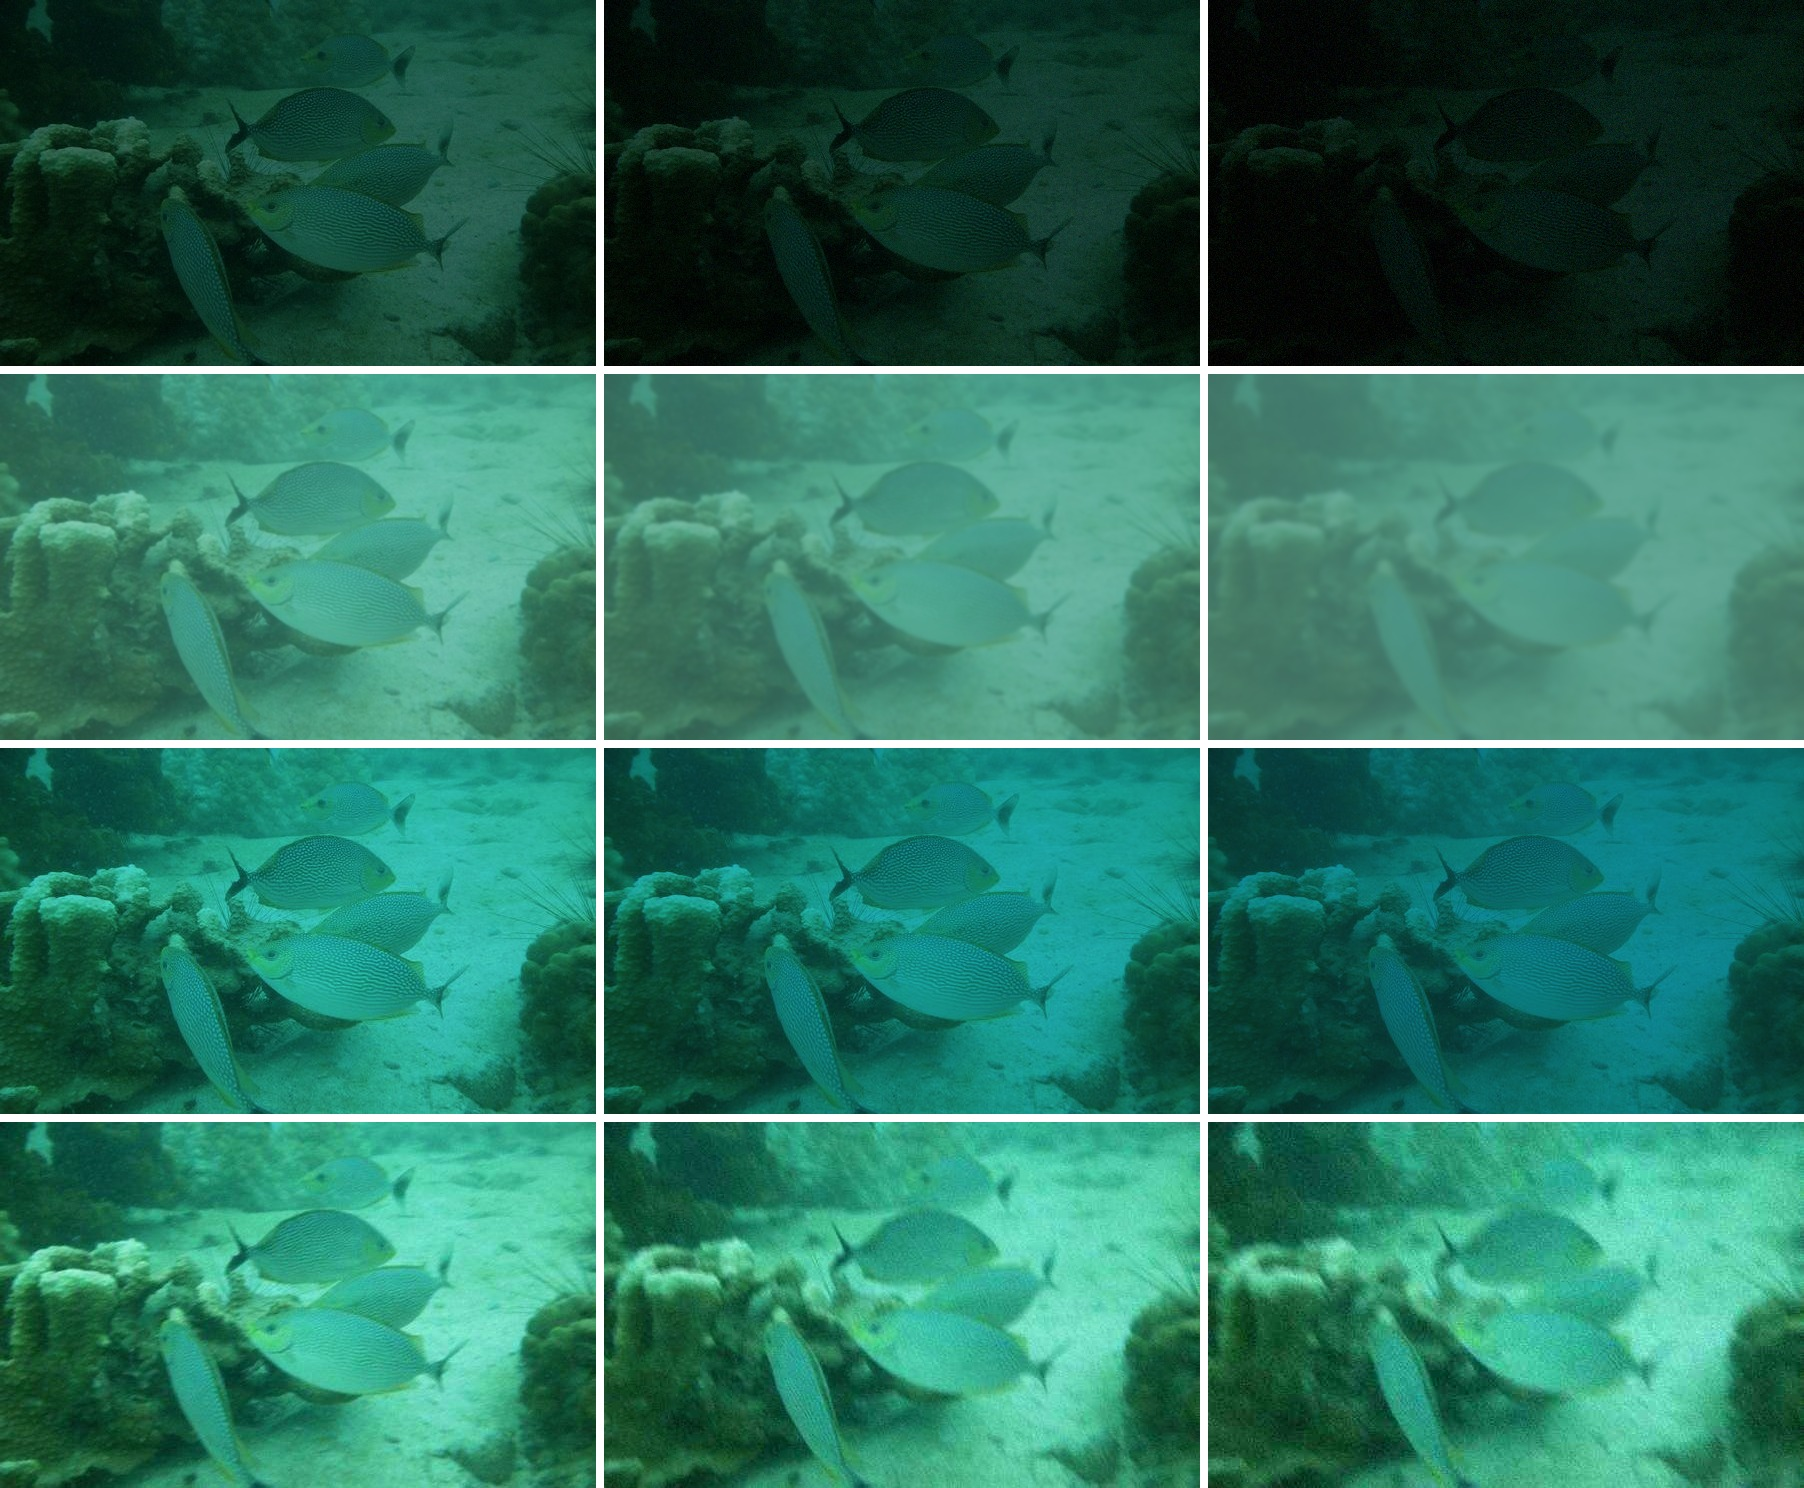
\includegraphics[width=0.65\textwidth]{figures/degradation_grid.jpg}
    \caption{Các biến dạng suy giảm nhân tạo áp dụng trên một ảnh test RUOD. Các hàng: dark, turbid, color cast, blur + noise; các cột: mức độ nghiêm trọng 1--3.}
    \label{fig:degradation_grid}
\end{figure}

\begin{table}[t]
    \centering
    \caption{mAP@0.5:0.95 dưới 12 điều kiện suy giảm trên tập test RUOD (\texttt{pycocotools}).}
    \label{tab:robustness}
    \resizebox{\columnwidth}{!}{
        \begin{tabular}{l c c c c c}
            \toprule
            Điều kiện        & Baseline A      & Semi-UIR B      & Đối chứng A150  & Đa miền C       & C $-$ A150 [CI 95\%]           \\
            \midrule
            Ảnh sạch         & 0,5991          & 0,5476          & 0,6151          & \textbf{0,6155} & +0,0027 [$-0{,}0003$, $+0{,}0056$] \\
            \midrule
            \texttt{dark1}   & 0,5386          & 0,4919          & 0,5431          & \textbf{0,5606} & +0,0181 [$+0{,}0146$, $+0{,}0218$] \\
            \texttt{dark2}   & 0,3041          & 0,3110          & 0,2632          & \textbf{0,3245} & +0,0664 [$+0{,}0611$, $+0{,}0717$] \\
            \texttt{dark3}   & 0,0555          & \textbf{0,0634} & 0,0402          & 0,0554          & +0,0295 [$+0{,}0247$, $+0{,}0346$] \\
            \texttt{turbid1} & 0,5824          & 0,4668          & 0,5861          & \textbf{0,5912} & +0,0067 [$+0{,}0034$, $+0{,}0100$] \\
            \texttt{turbid2} & 0,5060          & 0,3326          & 0,4867          & \textbf{0,5086} & +0,0193 [$+0{,}0150$, $+0{,}0234$] \\
            \texttt{turbid3} & \textbf{0,3099} & 0,1476          & 0,2738          & 0,3020          & +0,0274 [$+0{,}0220$, $+0{,}0323$] \\
            \texttt{cast1}   & 0,5824          & 0,5028          & 0,5939          & \textbf{0,6018} & +0,0072 [$+0{,}0039$, $+0{,}0102$] \\
            \texttt{cast2}   & 0,5587          & 0,4633          & 0,5662          & \textbf{0,5838} & +0,0165 [$+0{,}0130$, $+0{,}0198$] \\
            \texttt{cast3}   & 0,5303          & 0,4179          & 0,5349          & \textbf{0,5584} & +0,0248 [$+0{,}0210$, $+0{,}0287$] \\
            \texttt{blur1}   & 0,5028          & 0,4596          & 0,5142          & \textbf{0,5280} & +0,0175 [$+0{,}0141$, $+0{,}0215$] \\
            \texttt{blur2}   & 0,2709          & 0,2655          & 0,2768          & \textbf{0,3050} & +0,0251 [$+0{,}0199$, $+0{,}0304$] \\
            \texttt{blur3}   & 0,1064          & 0,1145          & 0,1212          & \textbf{0,1383} & +0,0093 [$+0{,}0036$, $+0{,}0148$] \\
            \midrule
            Tỷ lệ giữ lại TB & 66,8\%          & 61,4\%          & 65,0\%          & \textbf{68,5\%} & --                             \\
            \bottomrule
        \end{tabular}
    }
\end{table}

\begin{figure}[t]
    \centering
    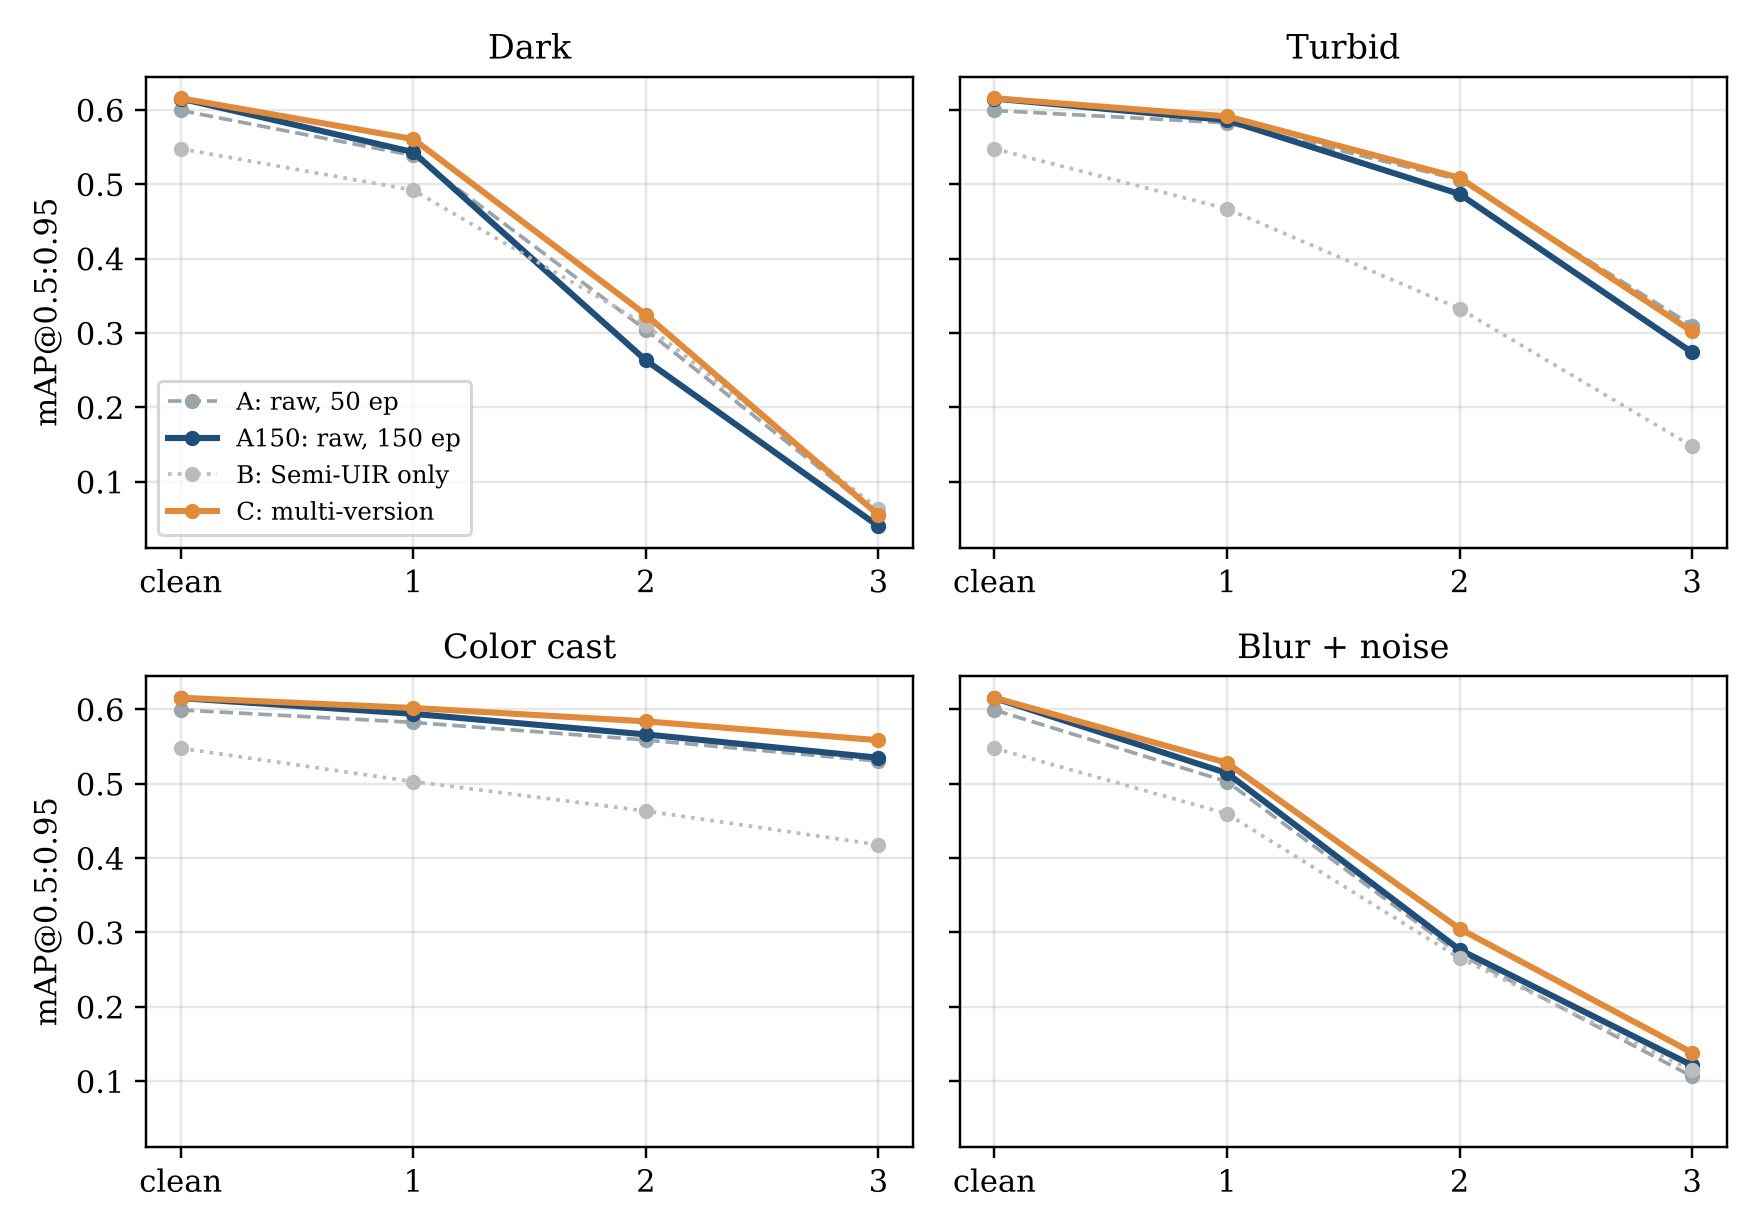
\includegraphics[width=0.65\textwidth]{figures/robustness_en.png}
    \caption{mAP@0.5:0.95 của bốn detector khi mức độ nghiêm trọng tăng dần đối với từng loại suy giảm (ảnh sạch = ảnh test không bị suy giảm).}
    \label{fig:robustness_curves}
\end{figure}

Như thể hiện ở Bảng~\ref{tab:robustness} và được biểu diễn theo mức độ suy giảm ở Hình~\ref{fig:robustness_curves}, Detector C vượt trội hơn Detector A150 ở cả 12 điều kiện suy giảm, với khoảng tin cậy 95\% paired bootstrap hoàn toàn trên 0 ($p_{\text{boot}} < 0{,}05$). Hình~\ref{fig:robustness_curves} thể hiện quỹ đạo suy giảm của 4 detector khi độ nghiêm trọng tăng dần: các mô hình đơn miền suy giảm nhanh chóng, trong khi huấn luyện đa phiên bản duy trì tỷ lệ giữ lại tốt hơn qua các mức biến dạng tăng dần. Tính trung bình qua tất cả các điều kiện, C giữ lại được 68,5\% mAP ban đầu, so với 65,0\% của A150. Detector B (chỉ học trên Semi-UIR) có tỷ lệ giữ lại thấp nhất (61,4\%); dù đạt mAP cao nhất ở điều kiện tối cùng cực (\texttt{dark3}, 0,0634) do Semi-UIR nâng sáng, mô hình này tụt sâu ở điều kiện nước đục (0,1476 ở \texttt{turbid3}) và ám màu.

Mức chênh lệch lớn nhất giữa C và A150 xuất hiện ở các mức suy giảm trung bình: ở \texttt{dark2}, C đạt 0,3245 so với 0,2632 của A150 (+0,0664, mức tăng tương đối 23\%); ở \texttt{turbid3}, C đạt 0,3020 so với 0,2738 (+0,0274).

Đáng chú ý, việc kéo dài thời gian huấn luyện đơn miền trên ảnh gốc làm detector kém bền đi. Mặc dù A150 tăng +0,0160 trên ảnh sạch so với baseline A, mô hình này lại tụt hậu so với A ở \texttt{dark2}, \texttt{dark3}, \texttt{turbid2} và \texttt{turbid3}. Ngược lại, huấn luyện đa miền giúp Detector C duy trì trọn vẹn độ chính xác trên ảnh sạch của A150, đồng thời xây dựng khả năng kháng chịu biến động môi trường mà không làm tăng độ trễ suy luận.

% ---------------------------------------------------------------------------
\section{Kết luận}
\label{sec:conclusion}

Chúng tôi đã khảo sát phương pháp tăng cường chọn lọc ảnh dưới nước cho bài toán phát hiện đối tượng với YOLO11n trên tập chuẩn RUOD.

Việc áp dụng đồng loạt SCNet hoặc Semi-UIR làm giảm mAP@0.5:0.95 đi 0,0026 và 0,0071 so với ảnh gốc. Bộ chọn ResNet18 (độ trễ 7,7\,ms) với ngưỡng $\tau = 0{,}625$ đạt mAP tương đương mốc ảnh gốc (0,6159 so với 0,6155), chủ yếu do giữ lại ảnh gốc ở 85,5\% trường hợp.

Oracle chọn giữa ảnh gốc và ảnh lật ngang đạt mức tăng +0,0207 mAP từng ảnh, bằng 144\% mức tăng của oracle quang học SCNet (+0,0144). Điều này cho thấy độ nhạy của detector trước các biến đổi không gian giải thích một phần đáng kể khoảng cách oracle lý thuyết. WBF 4 góc nhìn mang lại +0,0023 mAP trên toàn tập test (CI 95\% $[+0{,}0014, +0{,}0051]$).

Huấn luyện đa phiên bản nâng mAP@0.5:0.95 trên ảnh gốc từ 0,5990 lên 0,6155 so với baseline 50 epoch và ngang ngửa detector huấn luyện 150 epoch trên ảnh gốc (0,6150). Mô hình này còn vượt trội trên cả 12 điều kiện suy giảm chưa từng thấy, giữ lại 68,5\% mAP so với 65,0\%. Trong các thử nghiệm của chúng tôi, ảnh tăng cường mang lại giá trị thiết thực nhất khi được sử dụng làm dữ liệu huấn luyện đa miền để gia tăng độ bền môi trường, thay vì dùng làm lựa chọn theo từng ảnh lúc suy luận.

\enlargethispage{2\baselineskip}
\setlength{\bibitemsep}{0.1ex}
\printbibliography

\end{document}
